% ============================================================================
%  CHAPITRE 7 -- EXTENSIONS
% ============================================================================
\chapter{Extensions}
\label{chap:extensions}

\section{Transmission orientée tâche}
\label{sec:task}

Si le récepteur ne veut que l'étiquette, reconstruire l'image est un gaspillage. L'extension supprime le
décodeur image : un encodeur au stride 8 produit une carte latente réduite — $4\times4$ positions sur
CIFAR-10 — qui traverse le canal et alimente directement une tête de classification, entraînée par entropie
croisée.

\begin{table}[H]
\centering
\caption{Transmission orientée tâche sur CIFAR-10, AWGN (précision)}
\label{tab:task}
\small
\begin{tabular}{@{}lrrr@{}}
\toprule
\textbf{$k/n$} & \textbf{symboles / image} & \textbf{\SI{0}{\decibel}} & \textbf{\SI{10}{\decibel}} \\
\midrule
$1/384$ & 8  & 57,4\,\% & 70,5\,\% \\
$1/48$  & 64 & 72,4\,\% & 76,9\,\% \\
\midrule
\multicolumn{2}{@{}l}{\emph{Rappel : JSCC sémantique à $1/12$}} & 56,4\,\% & 78,2\,\% \\
\bottomrule
\end{tabular}
\end{table}

À $1/384$, soit \textbf{32 fois moins de bande} que le JSCC complet, la précision atteint 70,5\,\% contre
78,2\,\%. À $1/48$ elle atteint 76,9\,\%. À \SI{0}{\decibel}, avec 8 symboles seulement, le système orienté
tâche fait déjà mieux (57,4\,\%) que le JSCC sémantique complet (56,4\,\%).

\begin{figure}[H]
  \centering
  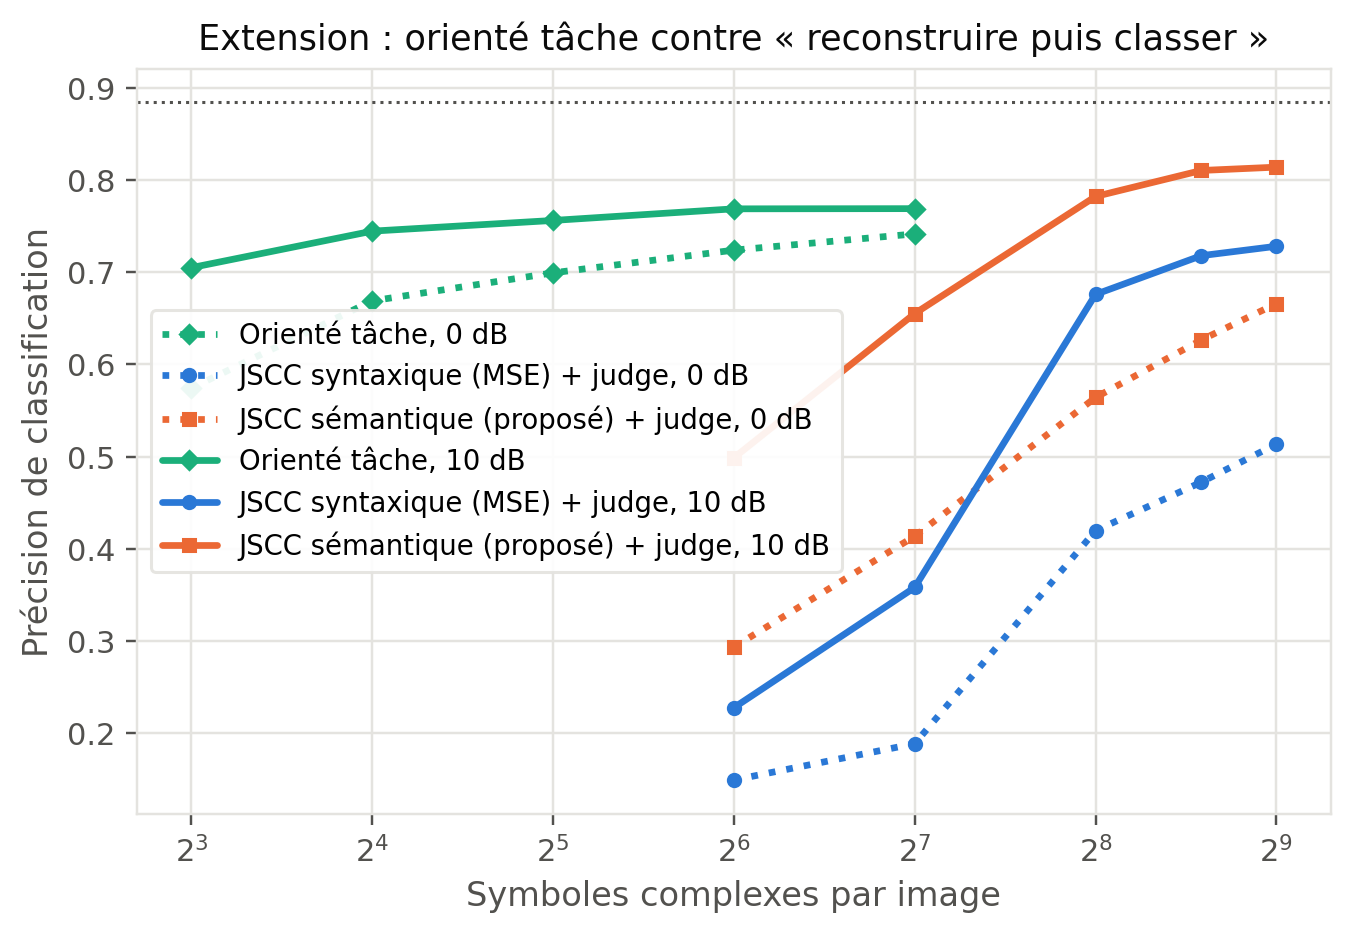
\includegraphics[width=0.88\linewidth]{task_oriented.png}
  \caption{Orienté tâche contre « reconstruire puis classer », en fonction du nombre de symboles par image.}
  \label{fig:task}
\end{figure}

\begin{keybox}[Interprétation]
L'information nécessaire à une décision parmi dix classes est très inférieure à celle qui décrit une image.
La contrepartie est l'absence de polyvalence : ce récepteur ne sait que classer, il ne peut pas afficher
l'image.
\end{keybox}

\section{Renouvellement conditionnel en vidéo}
\label{sec:cr}

Deux trames consécutives se ressemblent. L'extension envoie une image clé complète, puis uniquement les
\emph{blocs latents qui ont changé} ; le récepteur conserve les précédents pour les zones stables. La
signalisation des blocs renouvelés représente 12,7\,\% du débit et est comptée dans le rapport annoncé. Les
résultats correspondent à $\mathrm{frac} = 0{,}2$ et $c = 8$.

\begin{table}[H]
\centering
\caption{Renouvellement conditionnel contre transmission image par image, \SI{10}{\decibel}}
\label{tab:cr}
\small
\begin{tabularx}{\textwidth}{@{}lccc>{\raggedright\arraybackslash}X@{}}
\toprule
\textbf{Séquence} & \textbf{$k/n$ (CR)} & \textbf{PSNR CR} & \textbf{PSNR à $1/12$} & \textbf{Lecture} \\
\midrule
\srcfile{akiyo} (statique)           & $1/37$ & 26,40 & 26,48 & même qualité, 3 fois moins de bande \\
\srcfile{foreman} (modéré)           & $1/37$ & 25,15 & 28,06 & \SI{2.9}{\decibel} perdus \\
\srcfile{bus} (panoramique rapide)   & $1/37$ & 18,50 & 25,32 & \SI{6.8}{\decibel} perdus \\
\bottomrule
\end{tabularx}
\end{table}

\begin{figure}[H]
  \centering
  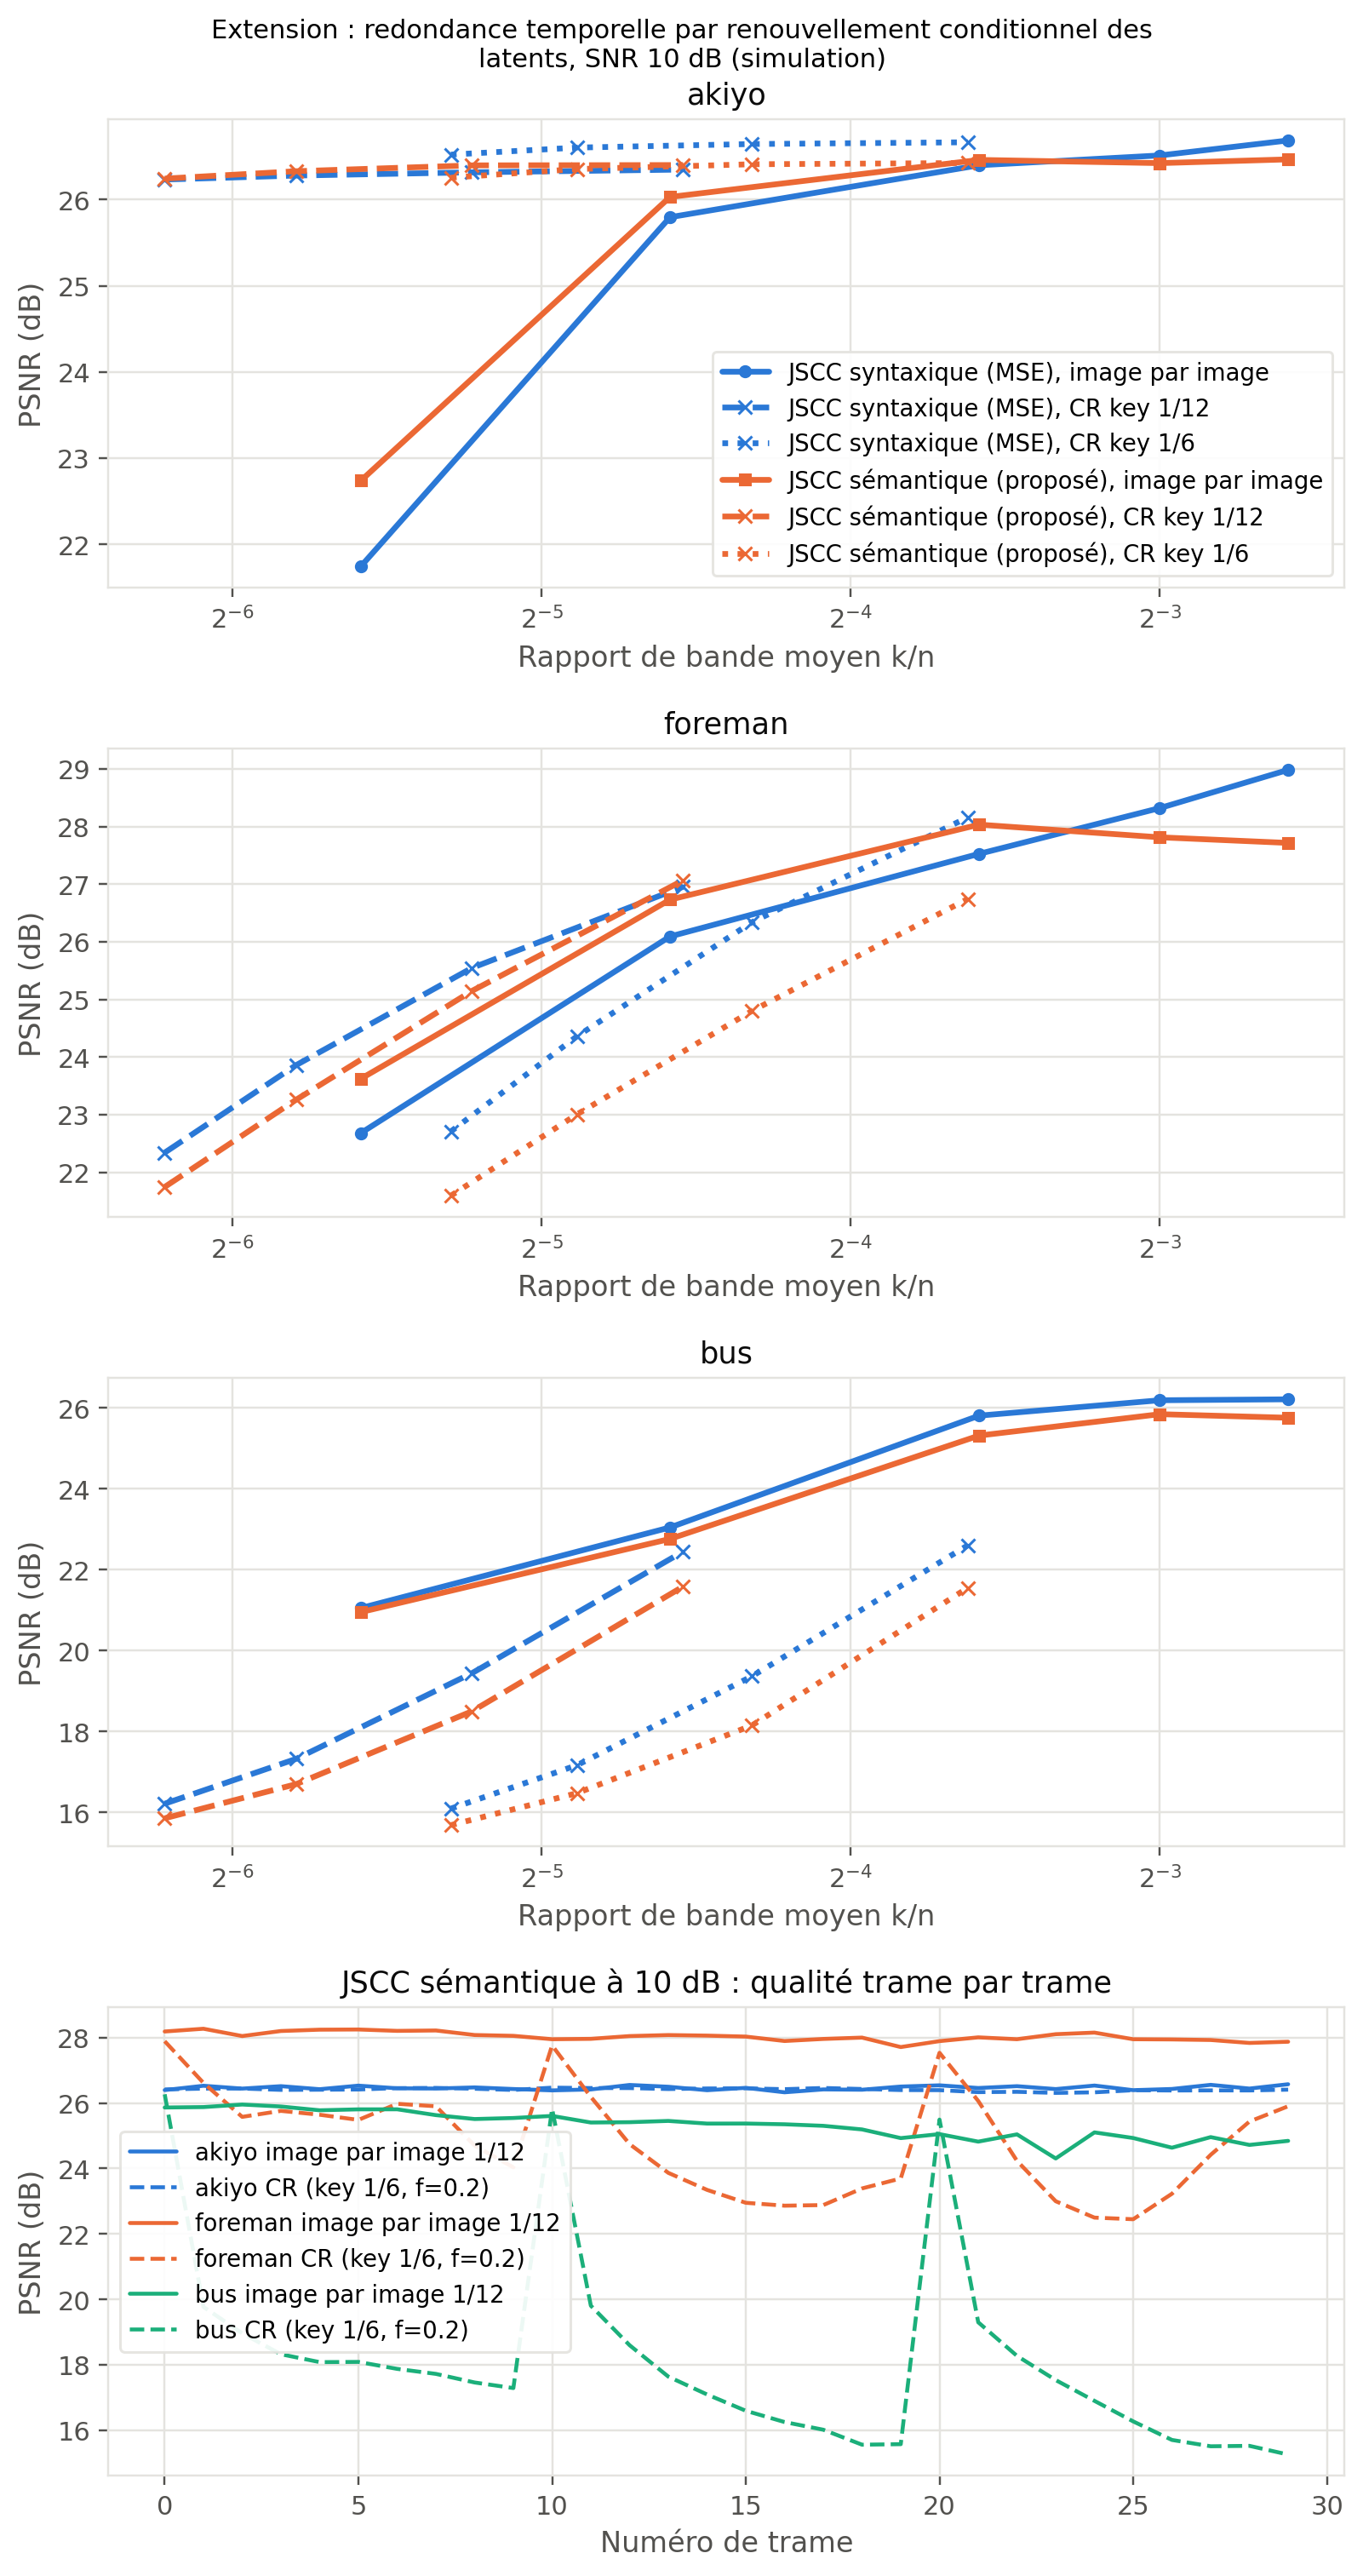
\includegraphics[width=0.76\linewidth]{video_rate.png}
  \caption{Débit effectivement utilisé au fil des trames, pour les trois régimes de mouvement.}
  \label{fig:video_rate}
\end{figure}

\begin{keybox}[Un résultat conditionnel]
La méthode exploite la redondance temporelle : elle n'apporte rien là où cette redondance n'existe pas. Le
résultat n'est pas « le renouvellement conditionnel fonctionne », mais « il fonctionne sur les scènes
statiques et doit être désactivé sur les scènes très mobiles ». Un système réel le piloterait par une mesure
de mouvement.
\end{keybox}
